% Created 2020-12-08 Tue 12:09
% Intended LaTeX compiler: pdflatex
\documentclass[a4paper,11pt,twoside]{article}
\usepackage[utf8]{inputenc}
\usepackage[T1]{fontenc}
\usepackage{graphicx}
\usepackage{grffile}
\usepackage{longtable}
\usepackage{wrapfig}
\usepackage{rotating}
\usepackage[normalem]{ulem}
\usepackage{amsmath}
\usepackage{textcomp}
\usepackage{amssymb}
\usepackage{capt-of}
\usepackage{hyperref}
\usepackage{minted}
\IfFileExists{./resources/style.sty}{\usepackage{./resources/style}}{}
\IfFileExists{./resources/referencing.sty}{\usepackage{./resources/referencing}}{}
\addbibresource{./resources/references.bib}
\usepackage[mode=buildnew]{standalone}
\usepackage{tikz}
\usetikzlibrary{decorations.fractals}
\usetikzlibrary{lindenmayersystems}
\author{Ryan Greenup \& James Guerra}
\date{\today}
\title{Spectral Analysis of Real Weighted Graphs}
\hypersetup{
 pdfauthor={Ryan Greenup \& James Guerra},
 pdftitle={Spectral Analysis of Real Weighted Graphs},
 pdfkeywords={},
 pdfsubject={},
 pdfcreator={Emacs 27.1 (Org mode 9.5)}, 
 pdflang={English}}
\begin{document}

\maketitle
\tableofcontents

 \newpage 

\begin{table}[htbp]
\centering
\begin{tabular}{lrll}
Headline & Time &  & \\
\hline
\textbf{Total time} & \textbf{8:31} &  & \\
\hline
Tasks & 8:31 &  & \\
\hspace*{2.0em}Derive the Sigmoid Curve &  &  & 4:00\\
\hspace*{1.0em}Derive and explain the equation on\ldots{} &  & 4:31 & \\
\end{tabular}
\caption{Clock summary at \textit{[2020-12-05 Sat 19:40]}}

\end{table}


\begin{quote}
\begin{center}
\begin{tabular}{ll}
Project Topic & \emph{Spectral Analysis of Real Weighted Graphs}\\
Adviser & Assoc. Prof. Laurence Park\\
\end{tabular}

\end{center}
\end{quote}

\begin{minted}[]{bash}
zotero & disown
kitty -e 'cd /home/ryan/Sync/Studies/2020ResearchTraining/spectral_analysis_graphs/' & disown
mattermost & disown
\end{minted}

\section{Tasks}
\label{sec:org99bde2d}
\subsubsection{Derive the Sigmoid Curve}
\label{sec:org7000edb}
Just make sure that you understand logistic regression so there is a ground-truth classification method.
\subsection{Derive and explain the equation on page 3}
\label{sec:orgaea1030}
RankNet is concerned with ranking things, the most obvious application of this
is information retrieval, for example if a search returns a variety of results
that are very similar to the query they will need to be ordered in some way to
make them more useful. This is traditionally done with \emph{PageRank} or by simply
using TF-IDF weighting, it is not immediately clear what advantages this
approach has, presumably it ranks results better.

The output of Ranknet is concerned with a probability of one object being ranked
higher than another and implements a Neural Network in order to model this. It
is not clear why RankNet is used for this rather than traditional classification
techniques.


Take two objects \(U_{i}, U_{j}\) (e.g. an article, document or anything else)
that are described by a feature vector \(\mathbf{X}_{i}\) and
\(\mathbf{X}_{j}\). RankNet maps this feature vector to some number:

\[
f: \mathbb{R}^{n} \rightarrow \mathbb{R}: \mathbf{X} \mapsto s
\]

If \(U_{i}\) is ranked higher than \(U_{j}\) this is denoted by:

\[
U_{i} \triangleright U_{j}
\]

The two outputs (\(s_{i}, s_{j}\)) are mapped to a probability that \(U_{i}\) is
ranked higher than \(U_{j}\) via a sigmoid function:

\[
p_{ij} \equiv P\left(U_{i} \triangleright U_{j} \right) \equiv \frac{1}{1 + e^{-\sigma \left(s_{i}-s_{j}\right)}} \label{eq:sigmoid}
\]

The model is dependent on the \(\sigma\) value as shown in figure \ref{fig:sig-animation}.


\url{media/sigmoid\_animation.gif}

In order to fit this curve a penalty term needs to be introduced to measure how well the curve fits the data. In regression analysis \(\mathrm{RMSE}=\sum_{i=1}^n \left[ \left(x_i - \hat{x}\right)^2 \right]\) is often used as loss function and could be implemented here.

Assume this is a binary classification problem (i.e. one is ranked higher) and
let \(p\) describe the probability of an object belonging to class 1. If an
observation belongs to class 1 we can measure the \emph{badness of fit} by \(1 - p\),
conversely if an object truly belongs to class 0 we can measure the badness of
fit by \(p\), this is illustrated in figure \ref{fig:residual_classification}.

\begin{table}[htbp]
\centering
\begin{tabular}{lll}
Actual Class & Residual & Cost\\
\(p=0\) & \(p\) & \(\ln{\frac{1}{1-p}}\)\\
\(p=1\) & \(1-p\) & \(\ln{\frac{1}{p}}\)\\
Either & \(p^{\left( 1- \overline{p} \right)\cdot  \left( 1- p \right)^{p}}\) & \(\ln{\left( p^{- p}\cdot  \left( 1- p \right)^{- \left( \overline{p} - 1 \right)} \right)}\)\\
\end{tabular}
\caption{\label{table:residuals}Residuals and costs function for}

\end{table}


\begin{figure}[htbp]
\centering
\includesvg[width=0.5\textwidth]{media/inkscape/classification_residual}
\caption{\label{fig:residual_classification}Residual from Classified points}
\end{figure}

These residuals (\(R\)) could be combined to account for either situation:


\begin{align}
      R= p^{1- \overline{p}}\cdot  \left( 1- p \right)^{\overline{p}}
\end{align}

A log transform would give a more convenient function (i.e. no exponents),
because the transform is monotone this will still work as a cost function and
so this could be implemented:

\begin{align}
     R^{*} = \left( 1- \overline{p} \right)\cdot  \ln\left( p \right) + \overline{p} \cdot  \ln\left( 1- p \right)
\end{align}

This however is not implemented in ranknet \cite{christopherburgesRankNetLambdaRankLambdaMART2010}, instead the cost function (\(C\)) satisfies the following property (see table \ref{table:residuals}):

\begin{align}
      \frac{1}{e^{C}} &= P_{ij}^{ \overline{P}_{ij}} \cdot  \left( 1- P_{ij} \right)^{\left( 1-\overline{P}_{ij} \right)} \\
       \iff C &= - \overline{P}_{ij} \ln\left( P_{ij} \right) - \left( 1 - \overline{P}_{ij} \right)\ln\left( 1- P_{ij} \right) \label{eq:cost}
\end{align}


Let the actual status of the ranking be defined by \(S_{i,j}\in \left\{-1, 0, 1\right\}\) like so:

\begin{center}
\begin{tabular}{rll}
\(S_{ij}\) & Status & Probability\\
1 & \(U_{i} \triangleright U_{j}\) & \(\overline{p}_{ij}=1\)\\
0 & \(U_{i} \enspace \square \enspace U_{j}\) & \(\overline{p}_{ij}=0.5\)\\
-1 & \(U_{i} \triangleleft U_{j}\) & \(\overline{p}_{ij}=0\)\\
 &  & \\
\end{tabular}

\end{center}

This provides that:

\begin{align}
      \overline{P}_{ij}= \frac{1}{2}\left( 1 +  S_{ij} \right) \label{eq:state}
\end{align}


The equations in \eqref{eq:sigmoid} and \eqref{eq:state} can be combined with \eqref{eq:cost} to give:


\begin{align}
    \overline{p} &= \frac{1}{2}\left( 1+ s \right) \label{eq:pbar} \\
    \log\left( p \right) &= - \log\left( 1 +  e^{- \sigma\left( s_i - s_j \right)} \right) \label{eq:logp} \\
    1- \overline{p} &= \frac{2}{2} - \frac{1+ s}{2} \label{eq:1mipbar}\\
    &= \frac{1- s}{2} \\
    \log\left( 1- p \right) &= \log\left( 1 -  \frac{1}{1 +  e^{- \sigma\left( s_i - s_j \right)}} \right) \\
    &= \log\left( \frac{1 +  e^{- \sigma\left( s_i - s_j \right)}-1}{1 +  e^{- \sigma\left( s_i - s_j \right)}} \right) \\
    &= \log \left( e^{- \sigma\left( s_i - s_j \right)} - \left( 1 +  e^{- \sigma \left( s_i - s_j \right)} \right)^{- 1} \right) \\
    &= - \sigma \left( s_i - s_j \right) - \log \left( 1 +  e^{- \sigma \left( s_i - s_j \right)} \right) \label{eq:logonemip}
\end{align}


The cost function from before was given by:

\begin{align}
    C &= - \overline{p} \log\left( p \right)- \left( 1 -  \overline{p} \right) \log\left( 1 - p \right) \\
\end{align}

so by comining \eqref{eq:pbar}, \eqref{eq:logp}, \eqref{eq:1mipbar} and \eqref{eq:eq:logonemip}:

\begin{align}
    C &= - \overline{p} \log\left( p \right)- \left( 1 -  \overline{p} \right) \log\left( 1 - p \right) \\
     &= \frac{1}{2}\left( 1 +  s \right)\log\left( 1 +  e^{- \sigma \left( s_i - s_j \right)} \right) - \frac{1- s}{2} \left( - \sigma \left( s_i - s_j \right) - \log\left( 1 +  e^{- \sigma \left( s_i - s_j \right)} \right) \right) \\
    &= \frac{1+ s}{2} \log\left( 1 +  e^{- \sigma\left( s_i - s_j \right)} \right) +  \frac{1- s}{2}\sigma \left( s_i - s_j \right)+  \frac{1- s}{2} \log \left(  1 +  e^{ -  \sigma \left( s_i - s_j \right)} \right) \\
    &= \log \left( 1 +  e^{ - `s \left( s_i - s_j \right)} \right) \left( \frac{1 +  s}{2} +  \frac{1 - s}{2} \right) +  \frac{1 - s}{2 `s \left( s_i - s_j \right)} \\
    &= \log \left( 1 +  e ^{- \sigma \left( s_i - s_j \right)}   \right) +  \frac{1 - s}{2 } \sigma \left( s_i -  s_j \right)
\end{align}



\subsection{Watch and summarise the Neural Networks Video}
\label{sec:org92a7cdf}
Create a Citation for this:
\begin{center}
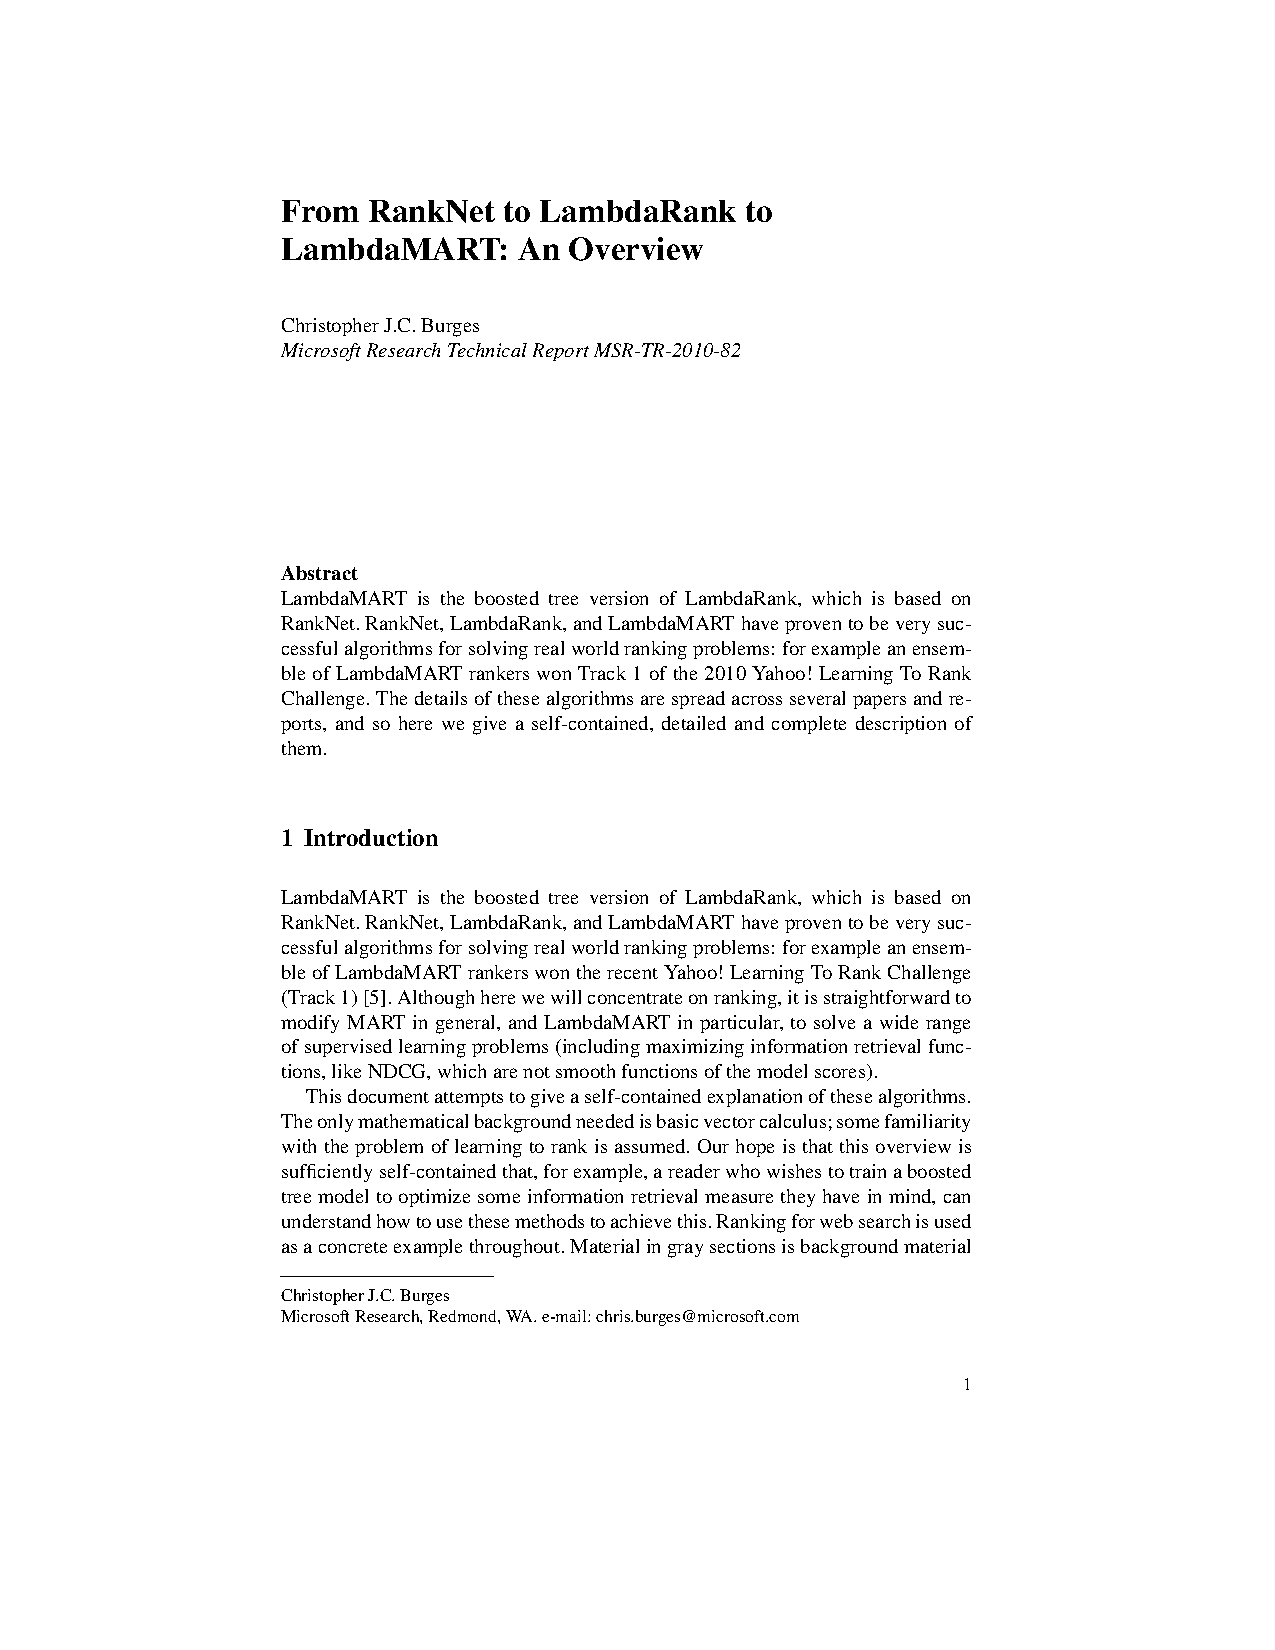
\includegraphics[width=.9\linewidth]{/home/ryan/Sync/Studies/2020ResearchTraining/spectral_analysis_graphs/resources/RankNet/RankNet_To_LambdaRank.pdf}
\end{center}

\subsection{Create a Neural Network to Classify binary data}
\label{sec:org8c1546f}

\begin{itemize}
\item Get the Data from UCI
\item Use three softwares to get an idea for it:
\begin{itemize}
\item \href{https://blog.rstudio.com/2020/09/29/torch/}{RTorch}
\item pytorch
\item JuliaTorch?
\end{itemize}
\end{itemize}

Compare the usability and performance of the different OS.
\subsection{Set up a Wiki and put the working in there}
\label{sec:org6274777}
And/or put the working into MkDocs Pages.
\subsection{Set up the wiki and comment on Mattermost}
\label{sec:org25b7f58}
\subsection{Add to the CDRMS Repo}
\label{sec:org75f642c}
\subsection{Set up Kanboard Page}
\label{sec:org3608499}
Share that page with Laurence.

This means that U\textsubscript{i} is ranked higher than U\textsubscript{j}
\subsection{Derive the sigmoid function for logistic regression}
\label{sec:orga7f3d7f}

\subsection{Clarify the Question}
\label{sec:org608fb0c}
\emph{Is there any benefit to using Ranknet rather than simply using Classification?}
\section{Ranknet}
\label{sec:orgfbe0e61}
The Ranknet uses a \href{../../../Notes/Org/roam/20201204180427-sigmoid\_curve.org}{Sigmoid Curve} curve:
\[
U_{i} \triangleright U_{j}
\]
\section{Summary}
\label{sec:org577425f}
\subsection{What is spectral Graph Theory}
\label{sec:orgafe5d5d}
Spectral graph theory starts by associating matrices to graphs, mostly the:


\begin{itemize}
\item Adjacency Matrix
\item Laplacian Matrix
\end{itemize}

\subsection{What do we mean by real weighted graphs}
\label{sec:org3b949ac}
Like non-integer values.
\subsection{What do I want to look at researching}
\label{sec:orgf44e580}
\subsection{What is the Research Outline}
\label{sec:org10c9cc6}
\subsubsection{This is what I put together in Planner}
\label{sec:org1698b8c}
\section{Research}
\label{sec:orgf25ebac}
\begin{itemize}
\item 
\end{itemize}



\subsection{Research Papers}
\label{sec:org9b366ad}

\begin{itemize}
\item Tu, E., Zhang, Y., Zhu, L., Yang, J., \& Kasabov, N., A Graph-Based Semi-Supervised k Nearest-Neighbor Method for Nonlinear Manifold Distributed Data Classification (). \cite{tuGraphBasedSemiSupervisedNearestNeighbor2016a}
\begin{itemize}
\item \href{file:///home/ryan/Sync/Studies/2020ResearchTraining/spectral\_analysis\_graphs/attachments/research/Enmei\_Tu\_Semi\_Supervised.pdf}{PDF}
\end{itemize}
\item Chang, S. Y., Pierson, E., Koh, P. W., Gerardin, J., Redbird, B., Grusky, D., \& Leskovec, J., Mobility network modeling explains higher SARS-CoV-2 infection rates among disadvantaged groups and informs reopening strategies (). \cite{changMobilityNetworkModeling2020}
\begin{itemize}
\item \href{file:///home/ryan/Sync/Studies/2020ResearchTraining/spectral\_analysis\_graphs/attachments/research/Serina\_Chang\_Mobility\_Networks.pdf}{PDF}
\end{itemize}
\end{itemize}


\subsection{Books}
\label{sec:orgd881d80}
\begin{itemize}
\item Bondy, J. A., \& Murty, U. S. R., Graph theory with applications (), : North Holland. \cite{bondyGraphTheoryApplications1976}
\begin{itemize}
\item \href{file:///home/ryan/Sync/Books/Textbooks/Mathematics/Data Science/GraphTheory/Graph\_Theory\_Bondy\_Murty.pdf}{PDF (local, absolute path)}
\end{itemize}
\item Nicodemi, O., Sutherland, M. A., \& Towsley, G. W., An introduction to abstract algebra with notes to the future teacher (), : Pearson Prentice Hall. \cite{nicodemiIntroductionAbstractAlgebra2007a}
\begin{itemize}
\item \href{file:///home/ryan/Sync/Books/Textbooks/Mathematics/Data Science/GraphTheory/Spectral\_Graph\_Theory}{Books on Spectral Graph Theory}
\end{itemize}
\end{itemize}





\section{Ring Theory\hfill{}\textsc{ATTACH}}
\label{sec:org6b9f292}
A rign is a set that has two operations (see \cite[\S\S 2.4-2.6]{nicodemiIntroductionAbstractAlgebra2007a}):

\begin{itemize}
\item Addition \((+)\)
\item Multiplication \(\cdot\)
\end{itemize}

And Satisfies the axioms of a ring:

\begin{enumerate}
\item Associativity of Addition

\(\left( \forall a,b,c \in \mathcal{R} \right) \left( a+ b \right) +  c = a +  \left(  b +  c    \right)\)
\end{enumerate}


\begin{enumerate}
\item Commutativity of Addition

\(\left( \forall a,b \in \mathcal{R}  \right) a +  b = b +  a\)

\item Additive Elements Exist

\(\left( \forall a \in \mathcal{R} \right) \wedge \left( \exists_0 \in \mathcal{R} \right) a +  0= 0 +  a =  a\)

\item Additive Inverse Exists

\(\left( \forall a \in \mathcal{R} \right)\wedge \left( \exists b \in \mathcal{R} \right) a +  b =  b +  a = 0\)

\begin{itemize}
\item This can be equivalently expressed:
\end{itemize}

\(\left( \forall a \in \mathcal{R} \right)\wedge \left( \exists \left( - a\right)\in \mathcal{R} \right) a +  \left( - a \right) = \left( - a \right) +  a = 0\)

\item Associativity of Multiplication

\(\left( \forall a,b,c, \in \mathcal{R} \right)\left( a \cdot  b \right)\cdot c = a \cdot  \left( b \cdot  c \right)\)
\end{enumerate}


\begin{enumerate}
\item Distributivity of Multiplication over Addition

\begin{itemize}
\item \(\left( \forall a,b,c, \in \mathcal{R} \right) \left( a\cdot  \left( b+ c \right)=  \left( a \cdot   b  \right) +  \left( a \cdot   c  \right) \right)\), AND
\item \(\left( \forall a,b,c, \in \mathcal{R} \right)\left( a +  b \right)\cdot   c = \left( a \cdot   c  \right)+  \left( b \cdot   c \right)\)
\end{itemize}
\end{enumerate}








\subsubsection{Further Axioms}
\label{sec:org6f11198}

Other conditions to have special classes of rings exist:

\begin{enumerate}
\item Commutativity of Multiplication
\begin{itemize}
\item A ring that satisfies this property is called a \textbf{commutative ring}

\(\left( \forall a,b \in \mathcal{R} \right) a \cdot  b = b \cdot  a\)
\end{itemize}

\item Existence of a Multiplicative Identity Element (A ring with Unity)
\begin{itemize}
\item A ring that satisfies this property is called a \textbf{ring with identity} or
\end{itemize}
equivalently a \textbf{ring with unity} (the multiplicative identity, often
denoted by \(1\), is called the \textbf{unity} of the ring.

\(\left( \exists 1 \in \mathcal{R} \right) \left( \forall a \in \mathcal{R} \right) 1 \cdot  a = a \cdot  1 = a\)
\end{enumerate}


\subsection{Integral Domain}
\label{sec:orgddb2a11}

An integral domain is a ring that:

\begin{enumerate}
\item is commutative
\item With identity/unity
\item Has no Zero Divisors
\end{enumerate}


In an integral domain we can cancel values:

\[
\left( c \neq 0 \right) \wedge \left( ac = bc \right)  \implies  a = b
\]

\subsection{Fields}
\label{sec:orga8552aa}

A field is:

\begin{enumerate}
\item An Integral Domain
\item In which every non-zero element is a unit
\end{enumerate}


A unit in a ring is an element of a ring that always has a multiplicative identity.
\end{document}
